\documentclass{beamer}
\usetheme{Boadilla}

\usepackage{standalone}
\usepackage[table]{xcolor}

\usepackage{fontspec}
\setmainfont{Times New Roman}

\usepackage[ukrainian]{babel}

\usepackage{polyglossia}
\setdefaultlanguage{ukrainian}
\setotherlanguages{english}
\setmonofont{Fira Code}[
  Scale=0.85
  ]
  \newfontfamily{\cyrillicfontsf}{Microsoft Sans Serif}

\usepackage{tikz}
\usepackage{pgfplots}
\usetikzlibrary{graphs,quotes}

\author{Кирило Байбула\\
        Науковий керівник:\\
        Самойленко Ігор Валерійович}
\date{\today}

\title{Знаходження оптимального шляху обміну у біржах на основі маркет мейкерів з функціями обміну константного добутку}

\institute{\textbf{КНУ ім. Тараса Шевченка}}

\date{\today}

\begin{document}

\begin{frame}
\titlepage{}
\end{frame}

\documentclass[beamer]{standalone}%

\begin{document}

\begin{frame}\frametitle{Що таке АММ?}
  \begin{block}{Автоматизовані Маркет Мейкери}
    АММ (або автоматизовані маркет мейкери) --- це механізм автоматизованого
    трейдингу електроними валютами, що визначений математичними формулами,
    законами, правилами.
  \end{block}

  \begin{figure}
    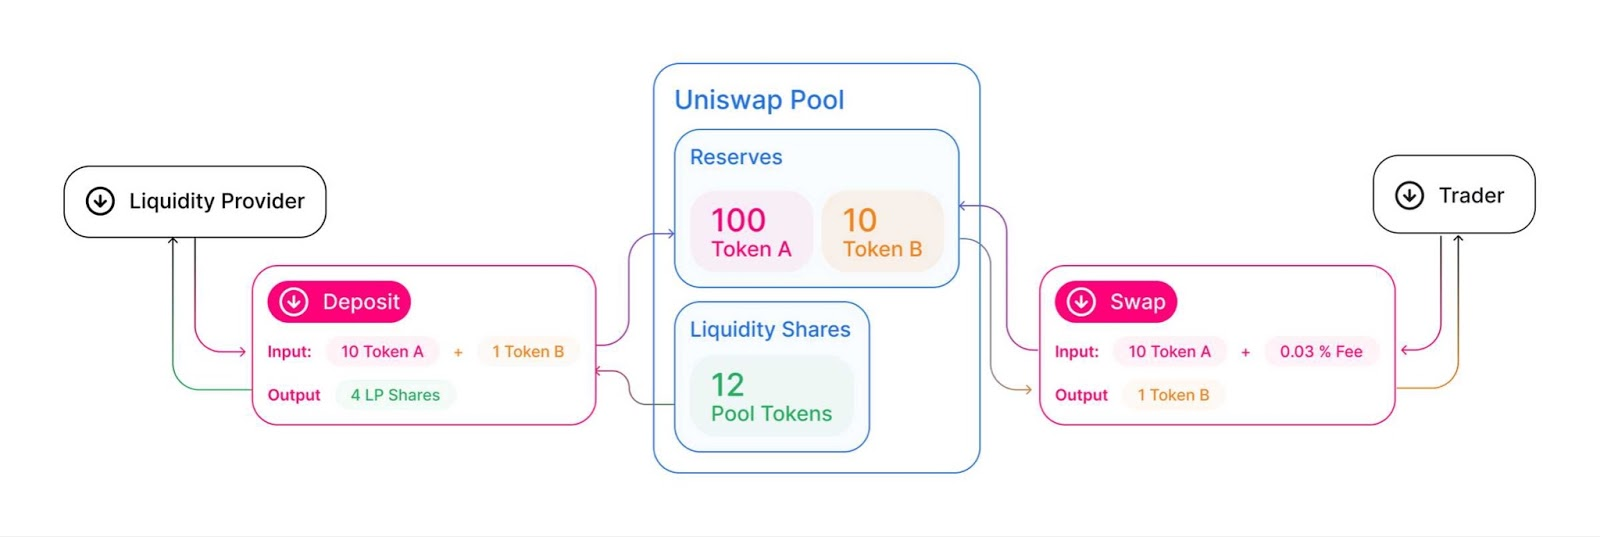
\includegraphics[scale=0.2]{./presentation/images/amm-intro-example.jpeg}
  \end{figure}
\end{frame}

\end{document}

\documentclass[beamer]{standalone}

\begin{document}

\begin{frame}\frametitle{У чому різниця між АММ та біржами на ордер буках?}
  \begin{block}{Order Book}
    Ордер Буки (з англ. \textit{order book}) --- це список заявок на купівлю та
    продаж активу, що відображається у вигляді таблиці з ціною та об'ємом.
  \end{block}
  \begin{columns}
    \column{0.5\textwidth}
    \begin{table}
      \begin{tabular}{ c | c }
        Об'єм & Ціна \\
        \hline \hline
        1 & 10,0 \\
        \rowcolor{red} 2 & 9,95 \\
        3 & 9,87 \\
        4 & 9,71
      \end{tabular}
      \caption{Таблиця на купівлю}
    \end{table}
    \column{0.5\textwidth}
    \begin{table}
      \begin{tabular}{ c | c }
        Ціна & Об'єм \\
        \hline \hline
        10,1 & 1 \\
        \rowcolor{green} 9,95 & 2 \\
        10,3 & 3 \\
        10,4 & 4
      \end{tabular}
      \caption{Таблиця на продаж}
    \end{table}
  \end{columns}
\end{frame}

\begin{frame}\frametitle{У чому різниця між АММ та біржами на ордер буках?}
  АММ для додатнього вектору вхідних об'ємів $\Delta \mathbf{x} \in \mathbb{R}^{n}$ та
  вихідних $\Delta \mathbf{y} \in \mathbb{R}^{n}$ визначає функцію
  $f(\Delta \mathbf{x}, \Delta \mathbf{y})$ над цими вкладами, що відповідає за визначення
  коректності трейду по правилам AMM.

  У випадку, якщо для даних $\Delta \mathbf{x}$ та $\Delta \mathbf{y}$ трейд вважається
  некоректним, то обмін не стається.
\end{frame}

\begin{frame}\frametitle{У чому різниця між АММ та біржами на ордер буках?}
  \begin{block}{Чим АММ краща за ордер буки?}
    \begin{itemize}
      \item Прозорість
      \item Детермінованість
      \item Простота в імплементації
    \end{itemize}
  \end{block}

  На цій моделі трейдингу побудовано багато децентралізованих бірж, таких як:

  \begin{itemize}
    \item Uniswap
    \item Curve
    \item SushiSwap
  \end{itemize}
\end{frame}

\end{document}

\documentclass[beamer]{standalone}%


\begin{document}

\begin{frame}\frametitle{Класифікація АММ}
  \begin{columns}
    \column{0.2\textwidth}
    \begin{tikzpicture}
      \node[draw] (amm) at (0, 0) {АММ};
      \node[draw] (cfmm) at (0, -2) {ММКФ};
      \node[draw] (cpmm) at (0, -4) {ММКД};

      \draw[->] (amm) -- (cfmm);
      \draw[->] (cfmm) -- (cpmm);
    \end{tikzpicture}

    \column{0.7\textwidth}
    \begin{block}{Автоматизовані маркет мейкери}
      \begin{equation*}
        \Delta x \in \mathbb{R} \, \Delta y \in \mathbb{R}
      \end{equation*}
    \end{block}

    \pause{}
    \begin{block}{Маркет мейкери константної функції}
      \begin{equation*}
        \varphi(R_{X} + \Delta x, R_{Y} - \Delta y) = \varphi(R_{X}, R_{Y})
      \end{equation*}
    \end{block}

    \pause{}
    \begin{block}{Маркет мейкери константного добутку}
      \begin{equation*}
        R_{X} \cdot R_{Y} = (R_{X} + \Delta x) \cdot (R_{Y} - \Delta y)
      \end{equation*}
    \end{block}
  \end{columns}
\end{frame}

\end{document}

\documentclass[beamer]{standalone}%


\begin{document}
\begin{frame}\frametitle{Крива резервів}

  \begin{tikzpicture}[domain=0:4]
    \begin{axis}%
      [
      grid=major,
      ticks=none,
      xlabel={$R_{X}$},
      ylabel={$R_{Y}$},
      axis x line=left,
      axis y line=left,
      no markers,
      domain=0:10,
      restrict y to domain=0:10000
      ]
      \addplot[thick,samples=400] (x,{10000/x});
    \end{axis}
  \end{tikzpicture}
\end{frame}

\begin{frame}\frametitle{Структура біржа на АММ}
\end{frame}

\end{document}

\input{presentation/frames/05_search_problem.tex}
\input{presentation/frames/06_solution.tex}

\end{document}
